\documentclass[tikz, border=4pt]{standalone}
\usepackage{tikz}
\usepackage{chemfig}
\begin{document}
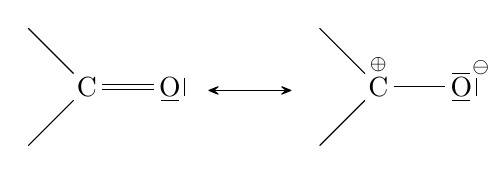
\begin{tikzpicture}[x=1cm, y=1cm]
  \node[anchor=north west, inner sep=0pt] at (0,0) {%
  \schemestart
    \chemfig{C([3]-)([5]-)=[@{db,.5}]@{atoo}\charge{0=\|,-90=\|}{O}}
    \arrow(.mid east--.mid west){<->}
    \chemfig{\charge{90:3pt=$\scriptstyle\oplus$}{C}([3]-)([5]-)-%
      \charge{0=\|,90=\|,-90=\|,45:3pt=$\scriptstyle\ominus$}{O}}
  \schemestop
  \chemmove{\draw[shorten <=2pt, shorten >=2pt](db) ..controls +(up:5mm) and +(up:5mm)..(atoo);}%
  };
\end{tikzpicture}
\end{document}
